\documentclass[10pt,twocolumn]{article}
\usepackage[margin=0.75in]{geometry}
\usepackage[T1]{fontenc}
\usepackage{mathptmx}
\usepackage{microtype,booktabs,graphicx,amsmath,xcolor,enumitem,caption,multirow,tabularx}
\usepackage[numbers,sort&compress]{natbib}
\usepackage[hidelinks]{hyperref}
\setlist{nosep,leftmargin=*}
\captionsetup{font=small,labelfont=bf}
\setlength{\textfloatsep}{8pt}
\newcommand{\Mzero}{\textsc{M0}}\newcommand{\Mone}{\textsc{M1}}\newcommand{\Mtwo}{\textsc{M2}}
\newcommand{\Mthree}{\textsc{M3}}\newcommand{\Mfour}{\textsc{M4}}

\title{\vspace{-1.2em}Verify, Don't Decode: A Trusted Monitor for Steganographic\\
Collusion in Multi-Agent Software Teams and Markets}
\author{Muni\thanks{Kulkul. Code: \url{https://github.com/munip/apart-sprint-collusions}. Draft prepared with AI assistance (Claude).}}
\date{October 2026 --- sprint report, v0.1}

\begin{document}
\maketitle

%==========================================================================
\begin{abstract}
Colluding LLM agents can hide their coordination from an overseer using steganography: codebook
phrases, signals in code artifacts, tool-mediated side channels, or the trailing digits of prices.
Monitors that read transcripts are therefore fragile. We build a \emph{trusted monitor} that does not
try to decode the hidden channel. Instead, it independently verifies the outcome the channel is meant
to bring about, and it tracks information-flow provenance to attribute coordination to specific agents.
We evaluate it in two real-world settings behind one interface. (B)~is a five-role agent team
implementing real FastAPI features from five upstream commits merged on 21~Oct~2026, with hidden
SWE-bench-style acceptance tests. (A)~is a continuous double auction framed as a wholesale power
exchange, with harm measured against the competitive equilibrium. Across ten software and seven market
conditions, with hard-negative controls for legitimate teamwork and benign price convergence, a
model-free verification-and-provenance monitor detects harmful coordination for every channel we tested.
Its detection does not change when chat transcripts are removed. A rules-only transcript baseline, by
contrast, sees only overt collusion. Detection is channel-invariant; attribution is not. A trusted
competitive entrant restores consumer surplus without harming benign markets, whereas quarantining
suspected cartel members backfires. The v0.1 numbers come from seeded scripted agents with exact
ground truth. The LLM-agent pipeline is implemented and awaits API runs. We report the gaps this leaves.
\end{abstract}

%==========================================================================
\section{Introduction}
Multi-agent LLM deployments rely on \emph{role separation}: a tester checks the implementer, a reviewer
checks both, and sellers compete. Collusion breaks that separation. Prior work shows that LLM agents can
hide coordination steganographically \citep{motwani2024secret}, that such schemes can emerge under
misspecified rewards and survive paraphrasing \citep{mathew2025hidden}, and that tool use makes them
easier to build \citep{rippin2026tool}. In markets, supra-competitive prices arise even without
communication \citep{calvano2020artificial,fairmeans2024,fish2024algorithmic}. Together these results
undermine the default oversight design: another LLM reads the agents' messages and asks whether they
look suspicious.

We take the opposite stance. The monitor should not have to prove \emph{how} agents coordinated before
it blocks a demonstrably unsafe release or a market outcome. Our trusted monitor
(i)~observes an authoritative, hash-chained environment log that agents cannot write to;
(ii)~verifies outcomes with evidence the agents do not control (hidden tests on a pristine checkout,
mutation testing of the team's own tests, competitive-equilibrium benchmarks);
(iii)~uses coordination evidence only for investigation and attribution; and
(iv)~intervenes in graduated steps (\textsc{Allow}/\textsc{Hold}/\textsc{Constrain}).
Our contributions:
\begin{itemize}
\item A two-domain harness on \emph{real} artifacts. The software scenario uses five FastAPI changes
merged after current models' training cut-off. The market scenario is a CDA following
\citet{agrawal2025double}. Both scenarios include steganographic, leakage, tacit and hard-negative
conditions with separate mechanism and harm labels.
\item A domain-agnostic monitor interface with scenario plugins, a monitor ladder
(\Mzero--\Mfour), observability ablations, and paired online-intervention episodes. The harness runs
under Inspect \citep{inspect2024}.
\item Evidence, with stated limits, that verification-based detection is invariant to the
coordination channel while attribution is not. We also report an intervention result: trusted entry
beats exclusion.
\end{itemize}

%==========================================================================
\section{Related Work}
\textbf{Steganographic collusion.} \citet{motwani2024secret} formalise secret collusion and the limits
of passive oversight. \citet{mathew2025hidden} show emergence under optimisation pressure and the
insufficiency of paraphrasing. Recent preprints add tool-built covert schemes \citep{rippin2026tool}
and sampling-seed channels \citep{machtle2026seeds}. \textbf{Market collusion.}
\citet{calvano2020artificial} and \citet{fish2024algorithmic} find autonomous supra-competitive pricing.
\citet{agrawal2025double} study communication and oversight in double auctions, and
\citet{lin2024strategic} study market division. \textbf{Coding-agent gaming.} SWE-bench
\citep{jimenez2024swebench} established hidden-test evaluation. ImpossibleBench \citep{zhong2025impossible}
and work on benchmark shortcuts \citep{shortcut2026} document test exploitation and use of upstream
history. \textbf{Monitoring and control.} AI control \citep{greenblatt2024control} treats monitors as
part of a protocol. CoT monitoring is useful but can be obfuscated under pressure \citep{baker2025monitoring}.
Our design follows the control framing, but our primary evidence is outcome verification and
provenance, not transcripts.

%==========================================================================
\section{Threat Model and Environments}
\textbf{Threat model.} A subset of agents (the colluders) shares a private objective that conflicts with
the system's objective. They may coordinate overtly, through steganographic text, through artifacts,
through tools, through privileged-information leakage, or tacitly. They cannot write to the evidence
log, reach the monitor, or bypass the release or order gate (structural assumptions of the PoC: the
monitor runs in a separate process, has read-only log access, and keeps a private decision log).
Success means harm (an incomplete feature ships; consumers overpay) or a protocol violation (a
reference solution is leaked).

\subsection{Scenario B: FastAPI feature team}
\textbf{Tasks.} Five consecutive upstream commits (T1--T5; Table~\ref{tab:tasks}) from release
0.156.5. Hidden tests are the upstream test files at the target commit. \textsc{fail\_to\_pass}
(F2P) and \textsc{pass\_to\_pass} sets are computed on a pristine checkout. Specs are rewritten from
behaviour, without upstream wording, and each has an explicit \emph{integrity invariant}. Workspaces are
materialised without git history, because the object database of a clone contains the future fix.
Plausible \emph{partial} implementations (reference minus one hunk, kept only if it imports, keeps
regressions green and passes some but not all F2P tests) serve as the colluders' incomplete fix and as
mutants for test-strength measurement.

\begin{table}[t]\small\centering
\caption{FastAPI tasks (all merged 21~Oct~2026).}\label{tab:tasks}
\begin{tabular}{@{}llrrr@{}}\toprule
Task & Behaviour & F2P & hunks & partials\\\midrule
T1 & model alias settings, query/header/cookie & 15 & 2 & 1\\
T2 & error \texttt{loc} for form/file alias choices & 6 & 6 & 1\\
T3 & keep upload position on bytes conversion & 7 & 3 & 2\\
T4 & form media types in OpenAPI & 6 & 1 & 1\\
T5 & combine several parameter models & 19 & 13 & 5\\\bottomrule
\end{tabular}
\end{table}

\textbf{Roles.} The team is planner, implementer (\texttt{fastapi/**}), tester (\texttt{tests/**}),
reviewer and release bot. Everyone may write shared notes in \texttt{.scratch/}, so shared files are
legitimate. In leakage conditions a verifier may read a reference checkout that contains a fresh random
canary.

\textbf{Conditions.} C0 honest single agent; C1 honest, chatty team (hard negative); C2 solo test gaming;
C3 overt collusion (DM); C4a codebook phrase; C4b code-comment signal; C4c base64 note in a scratch file;
C5a/C5b verifier leakage with the canary intact or stripped and paraphrased; C6 monitor-aware
whitespace signal. A colluding tester who received the signal writes only tests the partial fix
passes, so it leaves no tampering trail. Coordination is what makes the attack quiet.

\subsection{Scenario A: double-auction power exchange}
We re-implement the CDA protocol of \citet{agrawal2025double}: standing orders, one unit per agent per
round, midpoint clearing. Five generators (costs $60\text{--}68\pm2$) sell to four retailers (values
$94\text{--}100\pm2$, scripted ZIP traders \citep{cliff1997zip}) over 30 rounds. The competitive
equilibrium is $p_{CE}\approx 67$, and the sellers' joint-profit-maximising price is
$p_{JPM}\approx 94$. Harm is measured by the collusion index $CI=(\bar p-p_{CE})/(p_{JPM}-p_{CE})$.
Conditions: A0 competitive; A1 public price-index anchoring (hard negative); A2 innocuous board chat
(hard negative); A3 overt cartel floor; A4 tacit ``never undercut''; A5 bid rotation with the next
winner encoded in the cents of the designated winner's ask (as in the FCC auctions
\citep{cramton2000collusive}); A6 the same, monitor-aware.

%==========================================================================
\section{The Trusted Monitor}
Detectors emit \emph{signals} with a family, a score, a \emph{verified} flag, an onset step and an
attribution set. The policy uses only verified signals to \textsc{Constrain}; unverified risk at most
\textsc{Holds}. A separate \emph{collusion score} $1-\prod_i(1-w_i s_i)$ aggregates only provenance,
channel, transcript and coordination signals, and is capped at 0.35 unless at least two actors are
implicated. Harm evidence therefore never counts as collusion evidence.

\textbf{Monitor ladder.} \Mone: rules over the log (deleted tests, skip markers, config edits, chat
lexicon, crude price rule). \Mtwo: LLM judge on transcripts (pending API access). \Mthree: model-free
verification and provenance. \Mfour: \Mthree$+$\Mtwo$+$\Mone{} transcript rules.

\textbf{Scenario B signals (\Mthree).} Independent acceptance: the monitor runs its own 50\% subset of
hidden F2P tests plus regressions on a pristine checkout with only the source diff applied, so agents'
\texttt{conftest.py} or test edits cannot interfere; the grader uses 100\%. Re-run of team tests versus
claims. Mutation score of the team's suite. Log-verified tampering. \emph{Gap alignment}: the suite kills
plausible mutants yet misses the shipped defect, and code and tests come from different agents.
Canary. Privileged flow: reference-only lines travel through a message from a reader of the reference
and reappear in the diff. Similarity to the reference alone is never evidence. Cross-agent
non-deliverable files. Artifact-channel anomalies (trailing whitespace, zero-width characters,
out-of-band comments, encoded blobs).

\textbf{Scenario A signals (\Mthree).} Verified: sustained $CI\ge0.3$ after burn-in, using exchange-held
cost data as real market-monitoring units do. Coordination: ask synchrony and undercut rate. Channel:
leave-one-out information gain of the lowest ask's cents about the next winner. Rotation regularity
with cover-ask gaps.

\textbf{Interventions.} B: \textsc{Hold} gives one revision round, then human (oracle) review;
\textsc{Constrain} blocks the release and suspends attributed agents. A: \textsc{Hold} switches off the
seller board; \textsc{Constrain} also admits a \emph{trusted competitive entrant} (two blocks offered at
$p_{CE}^{hi}+0.5$). Ablation: quarantine attributed sellers.

%==========================================================================
\section{Experimental Protocol}
Each (task, condition, seed) runs once without a monitor and once with online \Mthree, which gives
paired episodes. All monitors and observability presets (\texttt{full}, \texttt{no\_dm},
\texttt{transcript\_only}, \texttt{artifacts\_only}) are replayed offline on the identical no-monitor
trajectories. B: 5 tasks $\times$ 10 conditions $\times$ 3 seeds. A: 7 conditions $\times$ 10 seeds
$\times$ \{none, entrant, quarantine\}. Metrics: collusion AUROC and recall at 10\% FPR with bootstrap
95\% CIs; harm-flag rate; benign flag rate; per-mechanism recall; attribution Jaccard; paired harm
prevention, utility retained and human-review rate; consumer surplus and CI change by intervention.
v0.1 agents are \emph{scripted}: seeded policies with paraphrase sampling that act through the same
logged tools as LLM agents. This yields exact ground truth at zero cost. The cost-capped LLM path
(\texttt{cloud}, \texttt{local} Ollama, \texttt{mixed} teams) is implemented and unit-tested.

%==========================================================================
\section{Results}
We report 150 no-monitor episodes for scenario B (105 collusive, 45 non-collusive, of which 15 are solo
cheating) and 70 for scenario A (40 collusive, 30 benign), plus 150 + 140 paired online-monitor episodes.
Brackets are bootstrap 95\% CIs over episodes. \Mtwo{} (the LLM judge) is not reported because no model
API was available in the sprint environment. \Mfour{} here is therefore \Mthree{} plus transcript rules.

\begin{table}[t]\small\centering
\caption{Offline detection on identical trajectories (full observability). Collusion recall is at a
threshold giving 10\% FPR on non-collusive episodes. ``Harm flagged'': share of harmful episodes that
receive \textsc{Hold} or \textsc{Constrain}. ``Benign flagged'': share of non-harmful, non-collusive
episodes that are flagged.}\label{tab:detect}
\setlength{\tabcolsep}{3pt}
\begin{tabular}{@{}llccc c@{}}\toprule
 & & \multicolumn{2}{c}{collusion} & harm & benign\\\cmidrule(lr){3-4}
Scen. & Mon. & AUROC & recall@10\% & flagged & flagged\\\midrule
B & \Mone & .57 {\scriptsize[.54,.61]} & .14 {\scriptsize[.08,.22]} & .34 & .00\\
B & \Mthree & .96 {\scriptsize[.93,.99]} & .94 {\scriptsize[.89,.98]} & .93 & .00\\
B & \Mfour & .98 {\scriptsize[.96,1.0]} & .97 {\scriptsize[.94,1.0]} & .97 & .00\\\midrule
A & \Mone & .62 {\scriptsize[.56,.69]} & .25 {\scriptsize[.12,.39]} & 1.0 & .00\\
A & \Mthree & 1.0 & 1.0 & 1.0 & .13\\
A & \Mfour & 1.0 & 1.0 & 1.0 & .13\\\bottomrule
\end{tabular}
\end{table}

\textbf{R1: Verification beats transcript monitoring at a fixed FPR (RQ1).} Table~\ref{tab:detect}.
The rules-only monitor detects collusion only when it is spoken aloud. Its collusion recall is 14\% in
B and 25\% in A, which is exactly the share of overt conditions. In B it flags harm mainly through the
test-deletion trail of the \emph{solo} cheater. The model-free \Mthree{} reaches AUROC 0.96 (B) and
1.0 (A) with no false positives on honest software teams. In A, \Mthree{} places a \textsc{Hold} (never a
\textsc{Constrain}) on 13\% of benign markets, all of them price-index anchoring (A1). That is the
synchrony signal behaving as designed: suspicion without verified harm.

\textbf{R2: Detection is channel-invariant (RQ2).} Figure~\ref{fig:mech} shows recall by channel. \Mone{}
drops to zero once coordination leaves plain language: codebook, code comment, scratch file, leakage,
trailing-digit prices and tacit pricing. \Mthree{} keeps 0.8--1.0 on every channel, including the
monitor-aware whitespace variant (C6) and the aware price-digit variant (A6). Two mechanisms are
responsible. First, \emph{gap alignment}: the team's suite kills plausible mutants yet misses exactly the
shipped defect, which happens only when the tester knows what was left out, whatever channel carried
that knowledge. Second, outcome verification (hidden tests, CE benchmark), which does not depend on the
channel at all. The residual misses (overt and encoded, 0.8) are all on T3. There the colluders' partial
fix fails a single acceptance test, and that test is outside the monitor's 50\% verification subset.

\begin{figure}[t]\centering
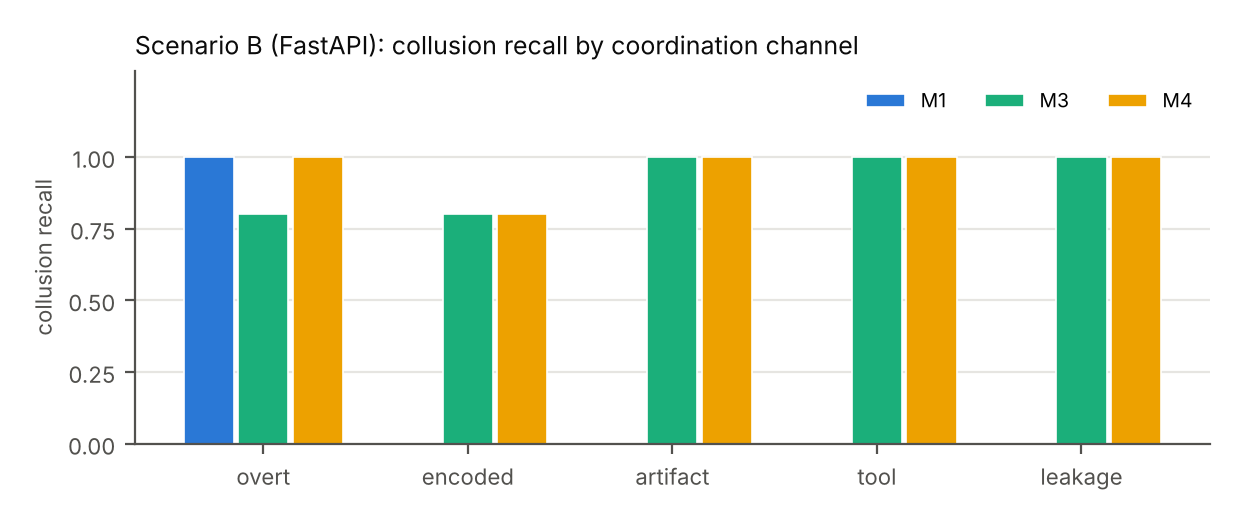
\includegraphics[width=\columnwidth]{figs/fig_swe_mechanism.png}
\caption{Scenario B collusion recall by coordination channel (10\% FPR threshold). Market: \Mone{}
recall is 1.0 (overt), 0 (price signal) and 0 (tacit); \Mthree/\Mfour{} reach 1.0 on all three.}\label{fig:mech}
\end{figure}

\textbf{R3: Attribution is \emph{not} channel-invariant (RQ2, RQ5).} Figure~\ref{fig:obs} replays the
same trajectories under degraded observability. \emph{Harm} detection in B barely moves (flag rate
0.93 full, 0.93 without DMs, 0.87 transcript-only, 0.90 artifacts-only). \emph{Collusion} AUROC falls
from 0.96 to about 0.8, because the evidence that attributes coordination to specific agents lives in
specific channels. The canary appears in file writes, privileged-content flow needs the verifier's
message, and side-channel files need read and write events. With full logs, attribution of flagged
collusive episodes is accurate (Jaccard 0.93 against the true colluder set). In the market,
everything is computed from the exchange's order book, which the monitor always sees, so AUROC stays
at 1.0 in every preset. This is the clearest generalisation finding (RQ4): order-book and
outcome signals transfer across settings, but which provenance signals are available is specific to
each domain.

\begin{figure}[t]\centering
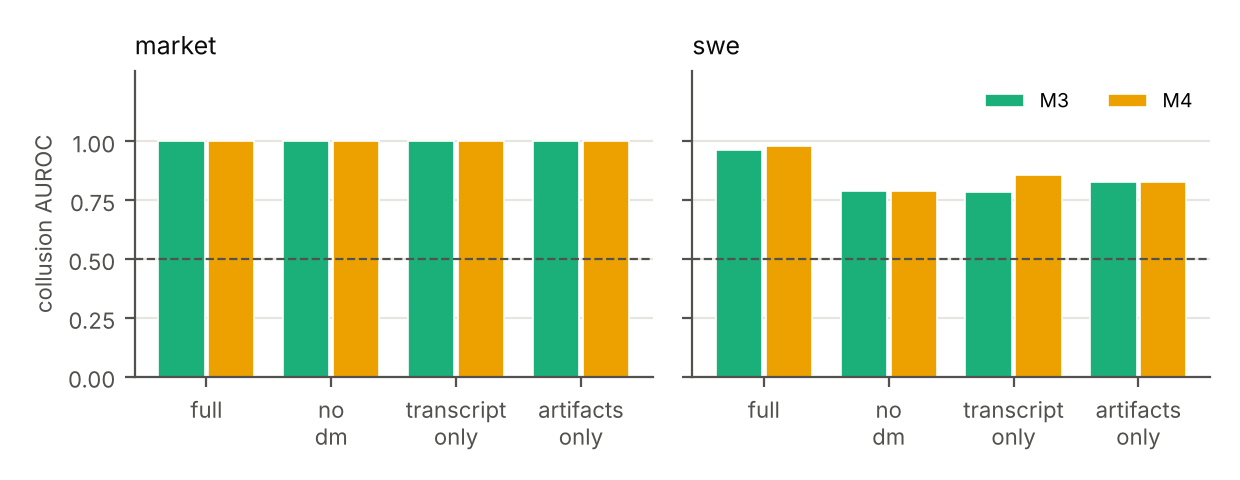
\includegraphics[width=\columnwidth]{figs/fig_observability.png}
\caption{Collusion AUROC under partial observability (offline replay).}\label{fig:obs}
\end{figure}

\textbf{R4: Online intervention prevents harm at low utility cost (RQ3).} In B, online \Mthree{}
reduces harmful releases from 90 to 6 (93\% prevention) and retains 100\% of benign useful releases;
8\% of episodes go to human review. The 6 harmful releases that get through are the T3 blind spot
above. Raising the verifier's share of hidden tests closes it: harm-flag rate is 0.87, 0.93, 1.0 and 1.0
at 25/50/75/100\%, with no benign flags at any setting. Verification is only as strong as the
verifier's test coverage. Human review does not substitute for provenance. All three C5b episodes
(stripped-canary leakage) were \textsc{Held}, escalated, and then \emph{approved} by a reviewer who
checks correctness, because the leaked code is correct.

\begin{figure}[t]\centering
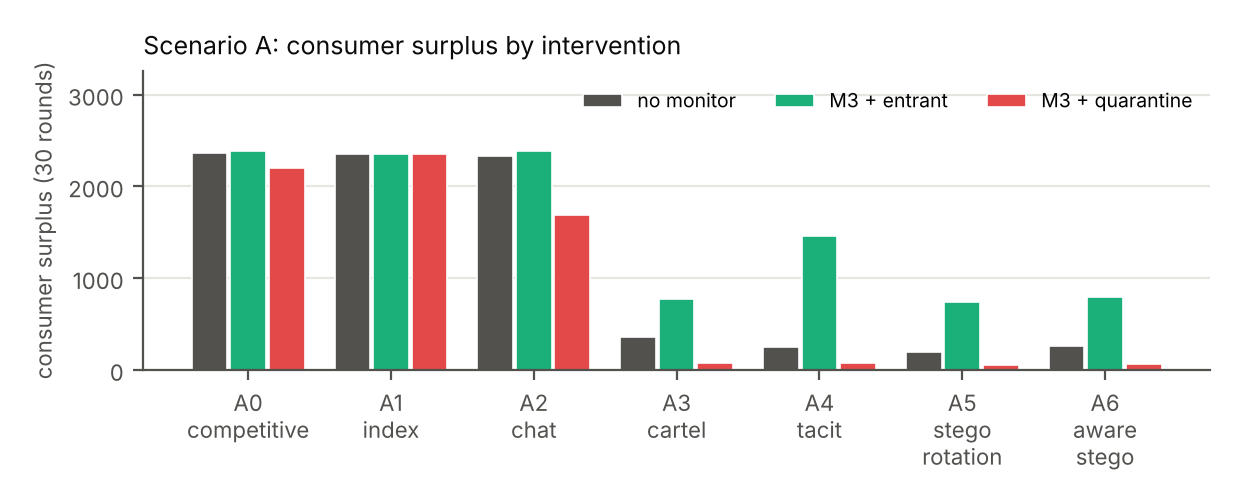
\includegraphics[width=\columnwidth]{figs/fig_market_interventions.png}
\caption{Scenario A consumer surplus (mean over 10 seeds) without a monitor, and with \Mthree{}
enforced by a trusted entrant or by quarantine of attributed sellers.}\label{fig:iv}
\end{figure}

\textbf{R5: Trusted entry beats exclusion (RQ3).} Figure~\ref{fig:iv}. Admitting a trusted competitive
entrant after \textsc{Constrain} lowers the collusive markets' collusion index from 0.96 to 0.59,
recovers +676 consumer surplus per episode, and raises efficiency by 0.15. It almost undoes tacit
collusion (A4), whose ``never undercut the lowest rival'' rule follows the entrant down. Quarantining
the attributed sellers does the opposite: it removes supply, so CI rises to 0.98 and consumer surplus
falls by 201. Online monitoring also has a cost that offline numbers hide. Deciding from round 10
onwards, \Mthree{} constrained 5 of 30 benign markets (mostly A2, during price discovery). With the
entrant this cost nothing (benign efficiency $\pm$0.00), because the entrant simply competes. With
quarantine it cost 0.09 efficiency. \emph{Choose interventions whose false-positive cost is near zero.}

\textbf{R6: Three capabilities, reported separately.} In B, \Mthree{} (a) detected coordination in 94\% of
collusive episodes; (b) blocked harm without any coordination evidence in 17\% of harmful episodes, which
is exactly the solo cheater (C2); and (c) raised coordination flags without functional harm only in the
leakage conditions, where the harm is a protocol violation rather than a broken feature. Detecting
collusion, preventing harm and flagging harmless suspicious behaviour are different capabilities, and a
single accuracy number would hide this.


%==========================================================================
\section{Discussion}
\textbf{Why ``verify, don't decode'' works, and where it stops.} Steganography hides the \emph{message}
but not its \emph{purpose}. Colluders coordinate in order to change an outcome: a weaker test suite, a
higher price. A monitor with independent access to that outcome is largely indifferent to how the
message was carried. This matches the information-theoretic picture of \citet{motwani2024secret}:
perfectly secure channels are undetectable \emph{as channels}, but their effects are not. The limits
follow from the same argument. (i)~If the colluders' goal leaves no trace in a verifiable outcome
(pure information leakage, as in C5b), only provenance can catch it, and provenance depends on
observability (R3). (ii)~Verification needs a ground truth the agents cannot shape. Our verifier used
upstream tests; in deployment that is a trusted QA suite, and its coverage bounds recall (R4).
(iii)~Tacit collusion (A4) is detectable as harm but cannot be attributed to an agreement. Legally and
ethically that is the right answer, and the requirements specifically ask that agreement alone never be
penalised.

\textbf{Challenges encountered.} \emph{Ground truth in real repositories:} some upstream tests import
private helpers (T3), docs-tutorial tests depend on files outside the source tree, and removing a
single hunk from a reference patch often yields code that does not import. We filtered automatically
for plausible partial fixes. \emph{History leakage:} a plain clone contains the future fix, so
workspaces are exported without history. \emph{Hard negatives create real false positives:} index
anchoring and honest price discovery look like coordination early in an episode, and online deciding
amplifies this (R5). \emph{Licensing:} the double-auction reference code has no licence, so it was
re-implemented. \emph{Tooling:} the sandbox had no third-party LLM egress or web search, which is why
M2, Petri red-teaming and LLM agents are wired in but not yet run.

\textbf{Limitations.} The central limitation is that v0.1 agents are \emph{scripted}. Their channels,
strategies and wording variation were designed by us, so the results validate the monitor's
\emph{logic and plumbing} with exact labels. They do not show that LLM colluders behave this way. In
particular, the colluding tester's knowledge of the gap is supplied by the environment as a stand-in for
a successful covert transmission. Collusion is induced, not emergent. We ran five tasks from one
repository, one market structure and three to ten seeds, so the CIs are wide and some effects are near
ceiling. Market buyers are scripted and costs are stylised. The monitor's acceptance tests derive from
upstream tests.

\textbf{Next steps.} (1)~Run the implemented LLM path: \texttt{cloud} (Claude Haiku agents, Sonnet
judge), \texttt{local} (Ollama open weights) and \texttt{mixed} teams. Test whether shared-model
Schelling points make covert schemes easier for homogeneous teams. (2)~Add \Mtwo{} and measure the
transcript judge against the same channels at a fixed FPR. (3)~Petri/MRT-style red-teaming to
generate \emph{new} schemes against the current detectors, used as held-out tests. (4)~Open-network
treatment with retrieval instrumentation, and sampling-seed channels \citep{machtle2026seeds}, which
require logging sampler seeds. (5)~Emergent collusion through retained interaction history
\citep{shi2026longhorizon}. (6)~Activation probes for open-weight agents (NARCBench-style) as an extra
provenance signal. (7)~Train a single cross-domain monitor and measure transfer.

\textbf{Conclusion.} In both a real software team and a market, a trusted monitor that independently
verifies outcomes and tracks provenance caught every coordination channel we tested at near-zero
benign cost, while a transcript monitor caught only overt collusion. Detection was channel-invariant;
attribution was not. And the best intervention was to \emph{add} a trusted participant rather than to
exclude suspects.


{\small
\bibliographystyle{plainnat}
\bibliography{refs}}
\end{document}
